\section{Fine structure in the LS-coupling scheme}

\begin{frame}{Fine structure in the LS-coupling scheme}
\uncover<1->{
    \begin{block}{Spin orbit coupling of electrons}
        Approximate calculations of relativistic quantum mechanics at low speeds: 
        \begin{equation*}
            U_{sl}=\frac{1}{2\mu^{2}c^{2}}\frac{1}{r}\frac{\mathrm{d}U}{\mathrm{d}r}\boldsymbol{s}\cdot\boldsymbol{l}=\xi(r)\boldsymbol{s}\cdot\boldsymbol{l}.
        \end{equation*}
    \end{block}}
\uncover<2->{
    The Hamiltonian:
    \begin{equation*}
        \begin{aligned}
            H_{\mathrm{s-o}}&=\sum_{i}\beta_i\boldsymbol{s}_i\cdot\boldsymbol{l}_i=\beta_{LS}\boldsymbol{S}\cdot\boldsymbol{L}.\\
            H&=H_{\mathrm{CF}}+H_{\mathrm{re}}+H_{\mathrm{s-o}}.
        \end{aligned}
    \end{equation*}}
\uncover<3->{
    the total electronic angular momentum: $\boldsymbol{J}=\boldsymbol{L}+\boldsymbol{S}$.
    \begin{gather*}
        \because\quad\boldsymbol{L}\cdot\boldsymbol{S}=\frac{\left(\boldsymbol{J}\cdot\boldsymbol{J}-\boldsymbol{L}\cdot\boldsymbol{L}-\boldsymbol{S}\cdot\boldsymbol{S}\right)}{2},\\
        \therefore\quad\left[\boldsymbol{J}^2,H\right]=0\quad\mathrm{~and~}\quad\left[{J}_z,H\right]=0.
    \end{gather*}
    }
\end{frame}

\begin{frame}{Fine structure in the LS-coupling scheme}
\uncover<1->{
    Therefore, $L_z, S_z$ are no longer conserved.
    \begin{equation*}
        \begin{aligned}
            \text{good quantum numbers}&: L,S,J,M_J,\\
            \text{eigenstates of} H&: \ket{LSJM_J}.
        \end{aligned}
    \end{equation*}}
\uncover<2->{
    The energy shift: (degeneracy with respect to $M_J$)
    \begin{equation*}
        \begin{aligned}
            E_{{\mathrm{s-o}}}&=\beta_{LS}\left\langle\boldsymbol{S}\cdot\boldsymbol{L}\right\rangle\\
            &=\frac{\beta_{LS}}{2}\left\{J\left(J+1\right)-L\left(L+1\right)-S\left(S+1\right)\right\}.
        \end{aligned}
    \end{equation*}}
\uncover<3->{
    \begin{block}{Lande interval rule}
        The energy interval between adjacent $J$ levels: 
        \begin{equation*}
            \Delta E_{{\mathrm{FS}}}=E_{J}-E_{J-1}=\beta_{LS}J\propto J.
        \end{equation*}
    \end{block}
    }
\end{frame}

\begin{frame}{Example: pp electronic configuration}
\only<1>{
    \begin{block}{$n\mathrm{p}n'\mathrm{p}\ (n\neq n')$}<1>
        \centering
        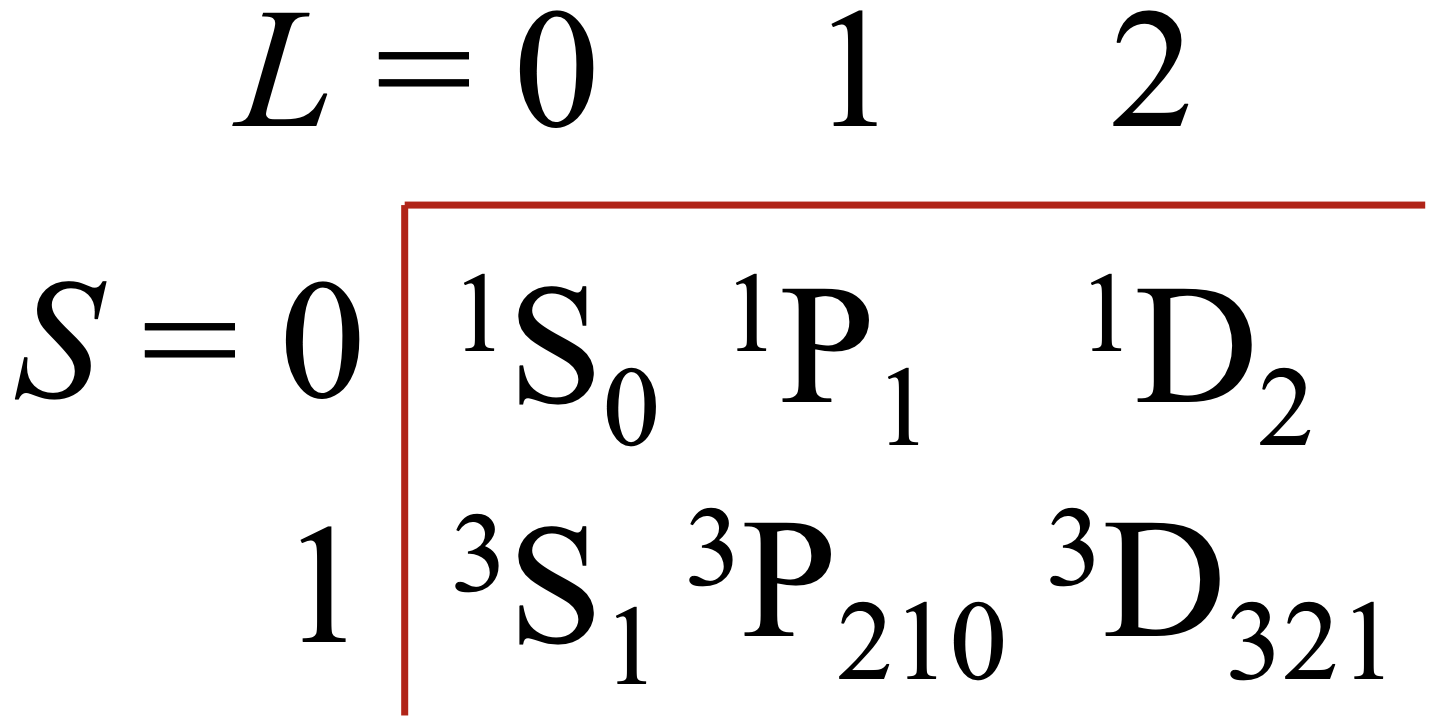
\includegraphics[scale=0.2]{fig/fig 5.3.png}
        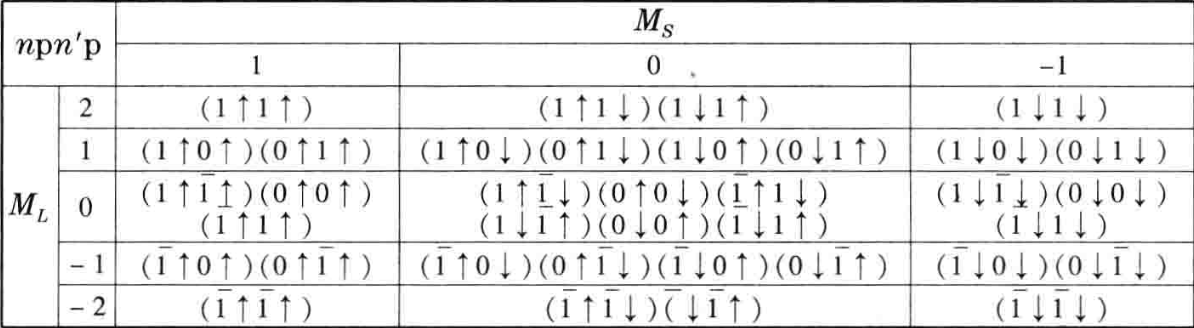
\includegraphics[scale=0.45]{fig/fig 5.4.png}
        \footnote{$\bar{1}=-1.$}
    \end{block}}
\only<2-3>{
    \begin{block}{$(n\mathrm{p})^2$}
        For equivalent electrons the Pauli exclusion principle restricts the states.
        \begin{center}
            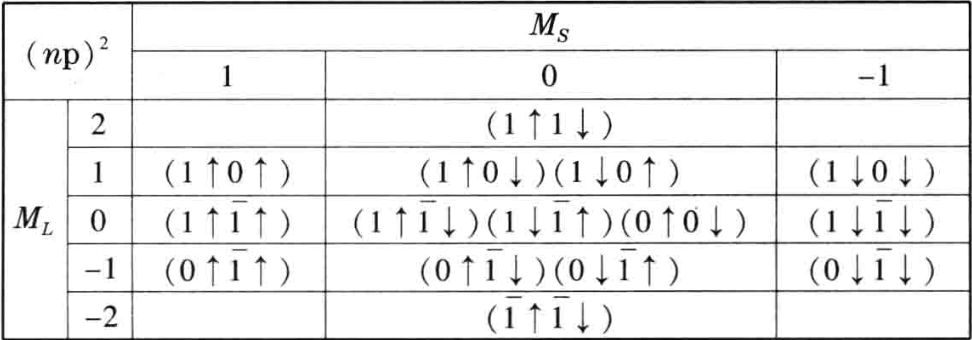
\includegraphics[scale=0.45]{fig/fig 5.5.png}
        \end{center}
        \begin{block}{Even rule:}<3>
            \begin{equation*}
                2|(L+S).
            \end{equation*}
        \end{block}
    \end{block}}
\only<4>{
    \begin{columns}
        \hspace*{1em}
        \column{0.47\textwidth}
            \begin{figure}
                \centering
                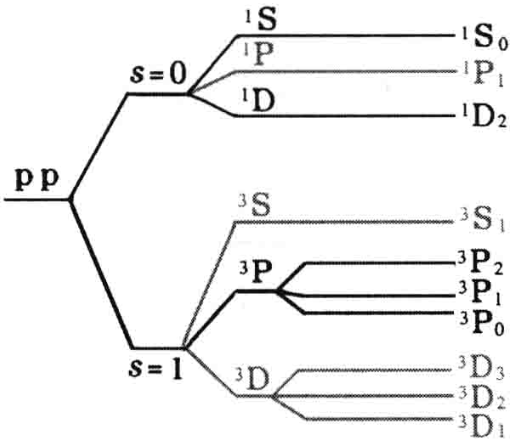
\includegraphics[scale=0.45]{fig/fig 5.6.png}
                \caption{pp electronic configuration energy levels}
            \end{figure}
        \column{0.54\textwidth}
            Black line: $(n\mathrm{p})^2$,\\
            Gray line: prohibited by Pauli's principle,\\
            All line: $n\mathrm{p}n'\mathrm{p}$.
    \end{columns}
}
\end{frame}

\begin{frame}{Hund's rules}
    \begin{block}{Hund's rules}
        \begin{enumerate}
            \item<1-> $S\nearrow\ E\searrow$;
            \item<2-> $L\nearrow\ E\searrow$;
            \item<3->
            \begin{itemize}
                \item<3-> Normal order ($J\searrow\ E\searrow$) : under half shell layer;
                \item<4-> Anomalous order ($J\nearrow\ E\searrow$) : over half shell layer.
            \end{itemize}
        \end{enumerate}
        \uncover<5->{However, Hund's rules are empirical and there are exceptions. They are more effective in inferring the ground state, with only a few exceptions. Using it to discuss excited states is not very reliable.}
    \end{block}
\uncover<6->{
    \begin{block}{Application: determine the ground state}
        \centering
        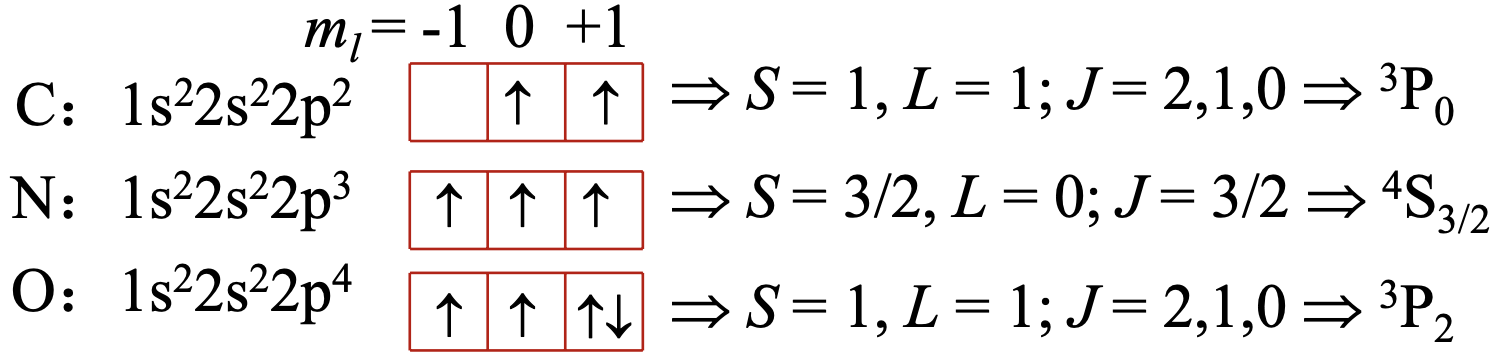
\includegraphics[scale=0.35]{fig/fig 5.7.png}
    \end{block}
    }
\end{frame}

\begin{frame}{Hund's rules}
    \begin{block}{Theoretical explanation}
    \uncover<1->{
        Generalize the potential expression of spin-orbit coupling to the coupling of any two angular momentum:
        \begin{equation*}
            U_{l_1l_2}=\frac1{2\mu^2c^2}\frac1r\frac{\mathrm{d}U}{\mathrm{d}r}{\boldsymbol{l}}_1\cdot{\boldsymbol{l}}_2,\quad (\boldsymbol{L}=\boldsymbol{l}_1+\boldsymbol{l}_2)
        \end{equation*}}
    \uncover<2->{
        The contribution of the coupling of angular momentum to the interaction potential: 
        \begin{equation*}
            \left\langle{\boldsymbol{l}}_1\cdot{\boldsymbol{l}}_2\right\rangle=\frac12\big[L(L+1)-l_1(l_1+1)-l_2(l_2+1)\big]\hbar^2.
        \end{equation*}}
    \uncover<3->{
        Apparently, $L\nearrow\ \left\langle{\boldsymbol{l}}_1\cdot{\boldsymbol{l}}_2\right\rangle\nearrow$, so the key is $\dfrac{\mathrm{d}U}{\mathrm{d}r}{~?~}0$.
        }
    \end{block}
\end{frame}

\begin{frame}{Hund's rules}
    \begin{block}{Theoretical explanation}
        \begin{itemize}
            \item<1-> Electron-electron Coulomb repulsion: 1\&2
            \begin{equation*}
                \frac{\mathrm{d}U}{\mathrm{d}r}\propto\frac{\mathrm{d}}{\mathrm{d}r}\left(\frac{e^2}{r}\right)\propto-\frac{1}{r^2}<0,
            \end{equation*}
            \item<2-> Electron-nucleon Coulomb attraction: 3-normal order
            \begin{equation*}
                \frac{\mathrm{d}U}{\mathrm{d}r}\propto\frac{\mathrm{d}}{\mathrm{d}r}\left(-\frac{e^2}{r}\right)\propto\frac{1}{r^2}>0,
            \end{equation*}
            \item<3-> Hole-nucleon Coulomb repulsion: 3-anomalous order
            \begin{equation*}
                \frac{\mathrm{d}U}{\mathrm{d}r}\propto\frac{\mathrm{d}}{\mathrm{d}r}\left(\frac{e^2}{r}\right)\propto-\frac{1}{r^2}<0.
            \end{equation*}
        \end{itemize}
    \end{block}
\end{frame}